\documentclass[twoside]{book}

% Packages required by doxygen
\usepackage{fixltx2e}
\usepackage{calc}
\usepackage{doxygen}
\usepackage[export]{adjustbox} % also loads graphicx
\usepackage{graphicx}
\usepackage[utf8]{inputenc}
\usepackage{makeidx}
\usepackage{multicol}
\usepackage{multirow}
\PassOptionsToPackage{warn}{textcomp}
\usepackage{textcomp}
\usepackage[nointegrals]{wasysym}
\usepackage[table]{xcolor}

% Font selection
\usepackage[T1]{fontenc}
\usepackage[scaled=.90]{helvet}
\usepackage{courier}
\usepackage{amssymb}
\usepackage{sectsty}
\renewcommand{\familydefault}{\sfdefault}
\allsectionsfont{%
  \fontseries{bc}\selectfont%
  \color{darkgray}%
}
\renewcommand{\DoxyLabelFont}{%
  \fontseries{bc}\selectfont%
  \color{darkgray}%
}
\newcommand{\+}{\discretionary{\mbox{\scriptsize$\hookleftarrow$}}{}{}}

% Page & text layout
\usepackage{geometry}
\geometry{%
  a4paper,%
  top=2.5cm,%
  bottom=2.5cm,%
  left=2.5cm,%
  right=2.5cm%
}
\tolerance=750
\hfuzz=15pt
\hbadness=750
\setlength{\emergencystretch}{15pt}
\setlength{\parindent}{0cm}
\setlength{\parskip}{3ex plus 2ex minus 2ex}
\makeatletter
\renewcommand{\paragraph}{%
  \@startsection{paragraph}{4}{0ex}{-1.0ex}{1.0ex}{%
    \normalfont\normalsize\bfseries\SS@parafont%
  }%
}
\renewcommand{\subparagraph}{%
  \@startsection{subparagraph}{5}{0ex}{-1.0ex}{1.0ex}{%
    \normalfont\normalsize\bfseries\SS@subparafont%
  }%
}
\makeatother

% Headers & footers
\usepackage{fancyhdr}
\pagestyle{fancyplain}
\fancyhead[LE]{\fancyplain{}{\bfseries\thepage}}
\fancyhead[CE]{\fancyplain{}{}}
\fancyhead[RE]{\fancyplain{}{\bfseries\leftmark}}
\fancyhead[LO]{\fancyplain{}{\bfseries\rightmark}}
\fancyhead[CO]{\fancyplain{}{}}
\fancyhead[RO]{\fancyplain{}{\bfseries\thepage}}
\fancyfoot[LE]{\fancyplain{}{}}
\fancyfoot[CE]{\fancyplain{}{}}
\fancyfoot[RE]{\fancyplain{}{\bfseries\scriptsize Generated by Doxygen }}
\fancyfoot[LO]{\fancyplain{}{\bfseries\scriptsize Generated by Doxygen }}
\fancyfoot[CO]{\fancyplain{}{}}
\fancyfoot[RO]{\fancyplain{}{}}
\renewcommand{\footrulewidth}{0.4pt}
\renewcommand{\chaptermark}[1]{%
  \markboth{#1}{}%
}
\renewcommand{\sectionmark}[1]{%
  \markright{\thesection\ #1}%
}

% Indices & bibliography
\usepackage{natbib}
\usepackage[titles]{tocloft}
\setcounter{tocdepth}{3}
\setcounter{secnumdepth}{5}
\makeindex

% Hyperlinks (required, but should be loaded last)
\usepackage{ifpdf}
\ifpdf
  \usepackage[pdftex,pagebackref=true]{hyperref}
\else
  \usepackage[ps2pdf,pagebackref=true]{hyperref}
\fi
\hypersetup{%
  colorlinks=true,%
  linkcolor=blue,%
  citecolor=blue,%
  unicode%
}

% Custom commands
\newcommand{\clearemptydoublepage}{%
  \newpage{\pagestyle{empty}\cleardoublepage}%
}

\usepackage{caption}
\captionsetup{labelsep=space,justification=centering,font={bf},singlelinecheck=off,skip=4pt,position=top}

%===== C O N T E N T S =====

\begin{document}

% Titlepage & ToC
\hypersetup{pageanchor=false,
             bookmarksnumbered=true,
             pdfencoding=unicode
            }
\pagenumbering{roman}
\begin{titlepage}
\vspace*{7cm}
\begin{center}%
{\Large A\+\_\+\+Star\+\_\+3D }\\
\vspace*{1cm}
{\large Generated by Doxygen 1.8.11}\\
\end{center}
\end{titlepage}
\clearemptydoublepage
\tableofcontents
\clearemptydoublepage
\pagenumbering{arabic}
\hypersetup{pageanchor=true}

%--- Begin generated contents ---
\chapter{Implementation of A$\ast$ Planning Algorithm in 3D Environment}
\label{md_readme}
\hypertarget{md_readme}{}
\href{https://travis-ci.org/VBot2410/A_Star_3D}{\tt } \subsection*{\href{https://coveralls.io/github/VBot2410/A_Star_3D?branch=master}{\tt } }

\subsection*{Overview}

A$\ast$ is a widely used algorithm for pathfinding in 2-\/D environments. This project takes the planning algorithm one step further and applies it to a 3-\/\+Dimensional environment.~\newline
 This project\textquotesingle{}s objective is to buid a planning module for Aerial Vehicles. Provided with the world boundary and Obstacle location data, the module provides the optimal path from start point to the goal by avoiding all obstacles.~\newline
 Development of this project follows {\bfseries Solo Iterative Process (S\+IP)} model in Software Engineering.~\newline
 Tested on Ubuntu 16.\+04 L\+TS with G\+CC 5.\+4.\+0.

\subsection*{Description}

The World boundary and obstacle data is provided in the (xmin,ymin,zmin,xmax,ymax,zmax) format. The module then uses this data along with the robot dimensions information to discretize the world and build a 3-\/D Configurtion Space. This C-\/\+Space is used to plan the Robot\textquotesingle{}s path using A$\ast$ Search. \paragraph*{A$\ast$ Search Algorithm}

A$\ast$ is an algorithm that searches for lowest cost path among all possible paths from start to goal. What A$\ast$ algorithm does is that at each step it picks the node from open list according to the value {\itshape f}, which is sum of two other parameters {\itshape g} and {\itshape h}. ~\newline
 Here, {\itshape g} value of a node is the cost to move from start to that node and {\itshape h} value is the estimated movement cost to move from that given node to the final destination.\+There are many ways to calculate {\itshape h} and this project provides an option to select between {\bfseries Euclidean Distance} and {\bfseries Manhattan Distance}.~\newline
 Obstacle nodes have the cost of infinity to travel through them and hence, the planner avoids these nodes in path planning.~\newline
 Typical implementations of A$\ast$ use a priority queue to perform the repeated selection of minimum (estimated) cost nodes to expand. This priority queue is known as the open list. At each step of the algorithm, the node with the lowest {\itshape f(x)} value is removed from the queue, the {\itshape f} and {\itshape g} values of its neighbors are updated accordingly, and these neighbors are added to the queue. The algorithm continues until a goal node has a lower {\itshape f} value than any node in the queue (or until the queue is empty). The {\itshape f} value of the goal is then the length of the shortest path, since {\itshape h} at the goal is zero in an admissible heuristic.

\subsection*{Solo Iterative Process (S\+IP)}


\begin{DoxyEnumerate}
\item Iteration 1\+:
\begin{DoxyItemize}
\item Planning of the Project Structure and Repository Setup.
\item Setup Travis and Coveralls.
\end{DoxyItemize}
\item Iteration 2\+:
\begin{DoxyItemize}
\item Build the Unit Testing Environment and Class Stubs.
\item Implementation of Map Builder and A$\ast$ \hyperlink{classPlanner}{Planner} with Fully working Path \hyperlink{classPlanner}{Planner}.
\item Release Version 1.\+0.
\end{DoxyItemize}
\item Iteration 3\+:
\begin{DoxyItemize}
\item Add Manhattan Distance Heuristic.
\item Explore the Possibility of 3-\/D Plots.
\item Release Version 2.\+0.
\end{DoxyItemize}
\item Iteration 4\+:
\begin{DoxyItemize}
\item Documentation.
\item Code Optimization.
\end{DoxyItemize}
\end{DoxyEnumerate}

Product and Iteration Backlogs can be found \href{https://docs.google.com/spreadsheets/d/1OG3C1JBhDQzr5JbrNKvgw2EXLqxJdgZZMIk44BRrPIw/edit?usp=sharing}{\tt Here}

U\+ML Diagrams can be found \href{https://github.com/VBot2410/A_Star_3D/tree/master/UML}{\tt Here}

\subsection*{Status}

$\sim$$\sim$\+Skeleton Code and Initial U\+ML Diagrams.$\sim$$\sim$~\newline
 $\sim$$\sim$\+Implementation of Map Builder from Environment Boundary and Obstacle Data.$\sim$$\sim$~\newline
 $\sim$$\sim$\+Implementation of A$\ast$ \hyperlink{classPlanner}{Planner}.$\sim$$\sim$~\newline
 $\sim$$\sim$\+Release Version 1.\+0 of the Module.$\sim$$\sim$~\newline
 {\bfseries Version 1.\+0 is Now Online.}

\subsection*{To Do (Version 2.\+0)}

Explore Possibility of 3-\/D Plots.~\newline
 Add Manhattan Distance Heuristic Function.~\newline
 Doxygen Comments and Documentation.~\newline


\#\# Build Instructions (Tested on Ubuntu 16.\+04 L\+TS with G\+CC 5.\+4.\+0.) 
\begin{DoxyCode}
1 git clone --recursive https://github.com/VBot2410/A\_Star\_3D
2 cd <path to repository>
3 mkdir build
4 cd build
5 cmake ..
6 make
7 
8 Run tests: ./test/A\_Star-test
9 Run program: ./app/A\_Star-app
\end{DoxyCode}
 \subsection*{License}

This Project is Licensed under the M\+IT License. Copy of the License Can be Found \href{https://github.com/VBot2410/A_Star_3D/blob/master/LICENSE}{\tt Here}

M\+IT License

Copyright (c) 2017 Vaibhav Bhilare 
\begin{DoxyCode}
1 Permission is hereby granted, free of charge, to any person obtaining a copy
2 of this software and associated documentation files (the "Software"), to deal
3 in the Software without restriction, including without limitation the rights
4 to use, copy, modify, merge, publish, distribute, sublicense, and/or sell
5 copies of the Software, and to permit persons to whom the Software is
6 furnished to do so, subject to the following conditions:
7 
8 The above copyright notice and this permission notice shall be included in all
9 copies or substantial portions of the Software.
10 
11 THE SOFTWARE IS PROVIDED "AS IS", WITHOUT WARRANTY OF ANY KIND, EXPRESS OR
12 IMPLIED, INCLUDING BUT NOT LIMITED TO THE WARRANTIES OF MERCHANTABILITY,
13 FITNESS FOR A PARTICULAR PURPOSE AND NONINFRINGEMENT. IN NO EVENT SHALL THE
14 AUTHORS OR COPYRIGHT HOLDERS BE LIABLE FOR ANY CLAIM, DAMAGES OR OTHER
15 LIABILITY, WHETHER IN AN ACTION OF CONTRACT, TORT OR OTHERWISE, ARISING FROM,
16 OUT OF OR IN CONNECTION WITH THE SOFTWARE OR THE USE OR OTHER DEALINGS IN THE
17 SOFTWARE.
\end{DoxyCode}
 
\chapter{Class Index}
\section{Class List}
Here are the classes, structs, unions and interfaces with brief descriptions\+:\begin{DoxyCompactList}
\item\contentsline{section}{\hyperlink{classBuild__Map}{Build\+\_\+\+Map} \\*\hyperlink{classBuild__Map}{Build\+\_\+\+Map} class declaration }{\pageref{classBuild__Map}}{}
\item\contentsline{section}{\hyperlink{structNode}{Node} \\*\hyperlink{structNode}{Node} of type Struct which Stores Various Property values of the Nodes }{\pageref{structNode}}{}
\item\contentsline{section}{\hyperlink{classPlanner}{Planner} \\*Declaration of Class \hyperlink{classPlanner}{Planner} }{\pageref{classPlanner}}{}
\item\contentsline{section}{\hyperlink{structVec3i}{Vec3i} \\*\hyperlink{structVec3i}{Vec3i} of type Struct which Builds points with x,y,z values }{\pageref{structVec3i}}{}
\end{DoxyCompactList}

\chapter{File Index}
\section{File List}
Here is a list of all documented files with brief descriptions\+:\begin{DoxyCompactList}
\item\contentsline{section}{app/\hyperlink{Build__Map_8cpp}{Build\+\_\+\+Map.\+cpp} \\*This File contains the code for \hyperlink{classBuild__Map}{Build\+\_\+\+Map} class which Discretizes the World using resolution values and marks obstacle positions in the workspace. Converts points from World to Discretized Workspace and vice versa }{\pageref{Build__Map_8cpp}}{}
\item\contentsline{section}{app/\hyperlink{main_8cpp}{main.\+cpp} \\*This project builds a discrete 3-\/D map from environment information and Implements the A$\ast$ algorithm to plan the path from Start to Goal Point }{\pageref{main_8cpp}}{}
\item\contentsline{section}{app/\hyperlink{Planner_8cpp}{Planner.\+cpp} \\*This file contains the code for \hyperlink{classPlanner}{Planner} Class which takes the Environment data built by the \hyperlink{classBuild__Map}{Build\+\_\+\+Map} Class and Uses A$\ast$ to plan the Shortest Path while avoiding all Obstacles }{\pageref{Planner_8cpp}}{}
\item\contentsline{section}{include/\hyperlink{Build__Map_8h}{Build\+\_\+\+Map.\+h} \\*This File contains the declarations of variables and methods for \hyperlink{classBuild__Map}{Build\+\_\+\+Map} class which Discretizes the World using resolution values and marks obstacle positions in the workspace. Converts points from World to Discretized Workspace and vice versa }{\pageref{Build__Map_8h}}{}
\item\contentsline{section}{include/\hyperlink{Planner_8h}{Planner.\+h} \\*This file contains the variables and function declarations for \hyperlink{classPlanner}{Planner} Class which takes the Environment data built by the \hyperlink{classBuild__Map}{Build\+\_\+\+Map} Class and Uses A$\ast$ to plan the Shortest Path while avoiding all Obstacles }{\pageref{Planner_8h}}{}
\end{DoxyCompactList}

\chapter{Class Documentation}
\hypertarget{classBuild__Map}{}\section{Build\+\_\+\+Map Class Reference}
\label{classBuild__Map}\index{Build\+\_\+\+Map@{Build\+\_\+\+Map}}


\hyperlink{classBuild__Map}{Build\+\_\+\+Map} class declaration.  




{\ttfamily \#include $<$Build\+\_\+\+Map.\+h$>$}

\subsection*{Public Member Functions}
\begin{DoxyCompactItemize}
\item 
\hyperlink{classBuild__Map_a1c1ffb3382a1c259bd139076e3ea2bf5}{Build\+\_\+\+Map} (std\+::vector$<$ double $>$, double, double, double)
\begin{DoxyCompactList}\small\item\em $<$ Public Access Specifier \end{DoxyCompactList}\item 
std\+::vector$<$ int $>$ \hyperlink{classBuild__Map_a4471712db8fbd8c8bc2fdefe8c0f551d}{World\+\_\+\+Dimensions} ()
\begin{DoxyCompactList}\small\item\em World\+\_\+\+Dimensions function returns the Discretized World Dimensions. \end{DoxyCompactList}\item 
std\+::vector$<$ int $>$ \hyperlink{classBuild__Map_ac702c59f16705f17230b565d998eecd3}{Build\+\_\+\+Obstacle} (std\+::vector$<$ double $>$)
\begin{DoxyCompactList}\small\item\em Build\+\_\+\+Obstacle Creates Obstacle Representations in Discretized Workspace given the Obstacle Blocks in World. \end{DoxyCompactList}\item 
std\+::vector$<$ int $>$ \hyperlink{classBuild__Map_a69943048bf44783d8413fa2a932225f7}{Build\+\_\+\+Node} (std\+::vector$<$ double $>$)
\begin{DoxyCompactList}\small\item\em Build\+\_\+\+Node creates the representation of a point from the world in Discretized Workspace. \end{DoxyCompactList}\item 
std\+::vector$<$ double $>$ \hyperlink{classBuild__Map_a9a0981707bd941c8b15a286ed5cff4aa}{Get\+\_\+\+Coordinate} (std\+::vector$<$ int $>$)
\begin{DoxyCompactList}\small\item\em Get\+\_\+\+Coordinate creates the representation of a point from location in the Discretized Workspace. \end{DoxyCompactList}\item 
virtual \hyperlink{classBuild__Map_a7e9cb965ff8a968a6c3c66b8411cbadc}{$\sim$\+Build\+\_\+\+Map} ()
\begin{DoxyCompactList}\small\item\em Destructor for Class \hyperlink{classBuild__Map}{Build\+\_\+\+Map}. \end{DoxyCompactList}\end{DoxyCompactItemize}
\subsection*{Public Attributes}
\begin{DoxyCompactItemize}
\item 
std\+::vector$<$ double $>$ \hyperlink{classBuild__Map_a56252a2d4d8971e370547cdb8a67eb8f}{Boundary}
\item 
std\+::vector$<$ int $>$ \hyperlink{classBuild__Map_ae65f595ae4825d69ae9e70d664beb644}{World}
\item 
double \hyperlink{classBuild__Map_a8aaaec9d533e5ea2c98045a7727389d7}{xy\+\_\+res}
\item 
double {\bfseries z\+\_\+res}\hypertarget{classBuild__Map_a23d568ed7281ff5682fc4fc94c366ea2}{}\label{classBuild__Map_a23d568ed7281ff5682fc4fc94c366ea2}

\item 
double {\bfseries margin}\hypertarget{classBuild__Map_ae3b0853f9e6e9b8b10e81babcee41b51}{}\label{classBuild__Map_ae3b0853f9e6e9b8b10e81babcee41b51}

\end{DoxyCompactItemize}


\subsection{Detailed Description}
\hyperlink{classBuild__Map}{Build\+\_\+\+Map} class declaration. 

\subsection{Constructor \& Destructor Documentation}
\index{Build\+\_\+\+Map@{Build\+\_\+\+Map}!Build\+\_\+\+Map@{Build\+\_\+\+Map}}
\index{Build\+\_\+\+Map@{Build\+\_\+\+Map}!Build\+\_\+\+Map@{Build\+\_\+\+Map}}
\subsubsection[{\texorpdfstring{Build\+\_\+\+Map(std\+::vector$<$ double $>$, double, double, double)}{Build_Map(std::vector< double >, double, double, double)}}]{\setlength{\rightskip}{0pt plus 5cm}Build\+\_\+\+Map\+::\+Build\+\_\+\+Map (
\begin{DoxyParamCaption}
\item[{std\+::vector$<$ double $>$}]{\+\_\+\+Boundary, }
\item[{double}]{\+\_\+xy\+\_\+res, }
\item[{double}]{\+\_\+z\+\_\+res, }
\item[{double}]{\+\_\+margin}
\end{DoxyParamCaption}
)}\hypertarget{classBuild__Map_a1c1ffb3382a1c259bd139076e3ea2bf5}{}\label{classBuild__Map_a1c1ffb3382a1c259bd139076e3ea2bf5}


$<$ Public Access Specifier 

Constructor for \hyperlink{classBuild__Map}{Build\+\_\+\+Map} Class.

Constructor


\begin{DoxyParams}{Parameters}
{\em Boundary} & has type double vector \& \{xmin,ymin,zmin,xmax,ymax,zmax\}format \\
\hline
{\em xy\+\_\+res} & has type double and stores x,y resolution \\
\hline
{\em z\+\_\+res} & has type double and stores z resolution \\
\hline
{\em margin} & has type double and stores the margin value for Robot Dimensions \\
\hline
{\em World} & has type double vector and stores World Dimensions \\
\hline
\end{DoxyParams}
$<$ X Dimension

$<$ Y Dimension

$<$ Z Dimension \index{Build\+\_\+\+Map@{Build\+\_\+\+Map}!````~Build\+\_\+\+Map@{$\sim$\+Build\+\_\+\+Map}}
\index{````~Build\+\_\+\+Map@{$\sim$\+Build\+\_\+\+Map}!Build\+\_\+\+Map@{Build\+\_\+\+Map}}
\subsubsection[{\texorpdfstring{$\sim$\+Build\+\_\+\+Map()}{~Build_Map()}}]{\setlength{\rightskip}{0pt plus 5cm}Build\+\_\+\+Map\+::$\sim$\+Build\+\_\+\+Map (
\begin{DoxyParamCaption}
{}
\end{DoxyParamCaption}
)\hspace{0.3cm}{\ttfamily [virtual]}}\hypertarget{classBuild__Map_a7e9cb965ff8a968a6c3c66b8411cbadc}{}\label{classBuild__Map_a7e9cb965ff8a968a6c3c66b8411cbadc}


Destructor for Class \hyperlink{classBuild__Map}{Build\+\_\+\+Map}. 

Destructor of \hyperlink{classBuild__Map}{Build\+\_\+\+Map} Class. 

\subsection{Member Function Documentation}
\index{Build\+\_\+\+Map@{Build\+\_\+\+Map}!Build\+\_\+\+Node@{Build\+\_\+\+Node}}
\index{Build\+\_\+\+Node@{Build\+\_\+\+Node}!Build\+\_\+\+Map@{Build\+\_\+\+Map}}
\subsubsection[{\texorpdfstring{Build\+\_\+\+Node(std\+::vector$<$ double $>$)}{Build_Node(std::vector< double >)}}]{\setlength{\rightskip}{0pt plus 5cm}std\+::vector$<$ int $>$ Build\+\_\+\+Map\+::\+Build\+\_\+\+Node (
\begin{DoxyParamCaption}
\item[{std\+::vector$<$ double $>$}]{Discrete}
\end{DoxyParamCaption}
)}\hypertarget{classBuild__Map_a69943048bf44783d8413fa2a932225f7}{}\label{classBuild__Map_a69943048bf44783d8413fa2a932225f7}


Build\+\_\+\+Node creates the representation of a point from the world in Discretized Workspace. 


\begin{DoxyParams}{Parameters}
{\em Discrete} & has type double vector \& contains x,y,z values of a point in World. \\
\hline
{\em Built\+\_\+\+Node} & has type integer vector \& contains representation of a point in Discretized Workspace \\
\hline
\end{DoxyParams}
\begin{DoxyReturn}{Returns}
Built\+\_\+\+Node of type integer vector 
\end{DoxyReturn}
\index{Build\+\_\+\+Map@{Build\+\_\+\+Map}!Build\+\_\+\+Obstacle@{Build\+\_\+\+Obstacle}}
\index{Build\+\_\+\+Obstacle@{Build\+\_\+\+Obstacle}!Build\+\_\+\+Map@{Build\+\_\+\+Map}}
\subsubsection[{\texorpdfstring{Build\+\_\+\+Obstacle(std\+::vector$<$ double $>$)}{Build_Obstacle(std::vector< double >)}}]{\setlength{\rightskip}{0pt plus 5cm}std\+::vector$<$ int $>$ Build\+\_\+\+Map\+::\+Build\+\_\+\+Obstacle (
\begin{DoxyParamCaption}
\item[{std\+::vector$<$ double $>$}]{v}
\end{DoxyParamCaption}
)}\hypertarget{classBuild__Map_ac702c59f16705f17230b565d998eecd3}{}\label{classBuild__Map_ac702c59f16705f17230b565d998eecd3}


Build\+\_\+\+Obstacle Creates Obstacle Representations in Discretized Workspace given the Obstacle Blocks in World. 


\begin{DoxyParams}{Parameters}
{\em v} & has type double vector \& contains obstacle boundary information \\
\hline
{\em Obstacle\+\_\+\+Extrema} & has type double vector \& contains the Obstale representation in Discretized Workspace \\
\hline
\end{DoxyParams}
\begin{DoxyReturn}{Returns}
Obstacle\+\_\+\+Extrema of type double vector 
\end{DoxyReturn}
\index{Build\+\_\+\+Map@{Build\+\_\+\+Map}!Get\+\_\+\+Coordinate@{Get\+\_\+\+Coordinate}}
\index{Get\+\_\+\+Coordinate@{Get\+\_\+\+Coordinate}!Build\+\_\+\+Map@{Build\+\_\+\+Map}}
\subsubsection[{\texorpdfstring{Get\+\_\+\+Coordinate(std\+::vector$<$ int $>$)}{Get_Coordinate(std::vector< int >)}}]{\setlength{\rightskip}{0pt plus 5cm}std\+::vector$<$ double $>$ Build\+\_\+\+Map\+::\+Get\+\_\+\+Coordinate (
\begin{DoxyParamCaption}
\item[{std\+::vector$<$ int $>$}]{Node\+\_\+\+Init}
\end{DoxyParamCaption}
)}\hypertarget{classBuild__Map_a9a0981707bd941c8b15a286ed5cff4aa}{}\label{classBuild__Map_a9a0981707bd941c8b15a286ed5cff4aa}


Get\+\_\+\+Coordinate creates the representation of a point from location in the Discretized Workspace. 


\begin{DoxyParams}{Parameters}
{\em Node\+\_\+\+Init} & has type integer vector \& contains representation of a point in Discretized Workspace \\
\hline
{\em Coordinates\+\_\+\+Generated} & has type double vector and contains x,y,z values of a point in World. \\
\hline
\end{DoxyParams}
\begin{DoxyReturn}{Returns}
Coordinates\+\_\+\+Generated of type double vector 
\end{DoxyReturn}
\index{Build\+\_\+\+Map@{Build\+\_\+\+Map}!World\+\_\+\+Dimensions@{World\+\_\+\+Dimensions}}
\index{World\+\_\+\+Dimensions@{World\+\_\+\+Dimensions}!Build\+\_\+\+Map@{Build\+\_\+\+Map}}
\subsubsection[{\texorpdfstring{World\+\_\+\+Dimensions()}{World_Dimensions()}}]{\setlength{\rightskip}{0pt plus 5cm}std\+::vector$<$ int $>$ Build\+\_\+\+Map\+::\+World\+\_\+\+Dimensions (
\begin{DoxyParamCaption}
{}
\end{DoxyParamCaption}
)}\hypertarget{classBuild__Map_a4471712db8fbd8c8bc2fdefe8c0f551d}{}\label{classBuild__Map_a4471712db8fbd8c8bc2fdefe8c0f551d}


World\+\_\+\+Dimensions function returns the Discretized World Dimensions. 

\begin{DoxyReturn}{Returns}
World of type integer vector \& contains Discretized World Dimensions 
\end{DoxyReturn}


\subsection{Member Data Documentation}
\index{Build\+\_\+\+Map@{Build\+\_\+\+Map}!Boundary@{Boundary}}
\index{Boundary@{Boundary}!Build\+\_\+\+Map@{Build\+\_\+\+Map}}
\subsubsection[{\texorpdfstring{Boundary}{Boundary}}]{\setlength{\rightskip}{0pt plus 5cm}std\+::vector$<$double$>$ Build\+\_\+\+Map\+::\+Boundary}\hypertarget{classBuild__Map_a56252a2d4d8971e370547cdb8a67eb8f}{}\label{classBuild__Map_a56252a2d4d8971e370547cdb8a67eb8f}
Boundary of type double vector, Stores World Boundary Data \index{Build\+\_\+\+Map@{Build\+\_\+\+Map}!World@{World}}
\index{World@{World}!Build\+\_\+\+Map@{Build\+\_\+\+Map}}
\subsubsection[{\texorpdfstring{World}{World}}]{\setlength{\rightskip}{0pt plus 5cm}std\+::vector$<$int$>$ Build\+\_\+\+Map\+::\+World}\hypertarget{classBuild__Map_ae65f595ae4825d69ae9e70d664beb644}{}\label{classBuild__Map_ae65f595ae4825d69ae9e70d664beb644}
World of type integer vector, Stores Discretized World Dimensions \index{Build\+\_\+\+Map@{Build\+\_\+\+Map}!xy\+\_\+res@{xy\+\_\+res}}
\index{xy\+\_\+res@{xy\+\_\+res}!Build\+\_\+\+Map@{Build\+\_\+\+Map}}
\subsubsection[{\texorpdfstring{xy\+\_\+res}{xy_res}}]{\setlength{\rightskip}{0pt plus 5cm}double Build\+\_\+\+Map\+::xy\+\_\+res}\hypertarget{classBuild__Map_a8aaaec9d533e5ea2c98045a7727389d7}{}\label{classBuild__Map_a8aaaec9d533e5ea2c98045a7727389d7}
x,y,z Resolutions and Robot Dimensions Margin Data of type double 

The documentation for this class was generated from the following files\+:\begin{DoxyCompactItemize}
\item 
include/\hyperlink{Build__Map_8h}{Build\+\_\+\+Map.\+h}\item 
app/\hyperlink{Build__Map_8cpp}{Build\+\_\+\+Map.\+cpp}\end{DoxyCompactItemize}

\hypertarget{structNode}{}\section{Node Struct Reference}
\label{structNode}\index{Node@{Node}}


\hyperlink{structNode}{Node} of type Struct which Stores Various Property values of the Nodes.  




{\ttfamily \#include $<$Planner.\+h$>$}



Collaboration diagram for Node\+:\nopagebreak
\begin{figure}[H]
\begin{center}
\leavevmode
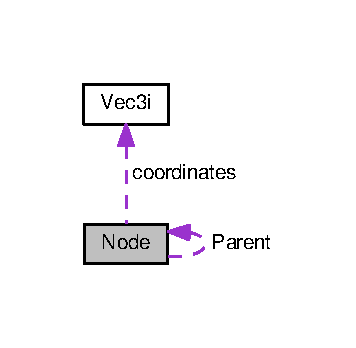
\includegraphics[width=171pt]{structNode__coll__graph}
\end{center}
\end{figure}
\subsection*{Public Member Functions}
\begin{DoxyCompactItemize}
\item 
\hyperlink{structNode_a947e5d8f76e9600c262ad97aefa67d8e}{Node} (\hyperlink{structVec3i}{Vec3i}, \hyperlink{structNode}{Node} $\ast$Parent\+\_\+=nullptr)
\begin{DoxyCompactList}\small\item\em Constructor for \hyperlink{structNode}{Node} Struct Initializes the \hyperlink{structNode}{Node} features to default values. \end{DoxyCompactList}\item 
double \hyperlink{structNode_a4a45812196b32f307390cd277953a6a0}{Get\+\_\+\+Score} ()
\begin{DoxyCompactList}\small\item\em Get\+\_\+\+Score function of return type double from \hyperlink{structNode}{Node} struct It Adds the G and H values of current node to give the F value. \end{DoxyCompactList}\end{DoxyCompactItemize}
\subsection*{Public Attributes}
\begin{DoxyCompactItemize}
\item 
double \hyperlink{structNode_aa6f89ef69e082186d2ab507ba1376940}{G}
\item 
double {\bfseries H}\hypertarget{structNode_a04d5df1c75751f4e12d745cf9415e672}{}\label{structNode_a04d5df1c75751f4e12d745cf9415e672}

\item 
\hyperlink{structVec3i}{Vec3i} \hyperlink{structNode_a5415b97e157699fceb6cd841c8767239}{coordinates}
\item 
\hyperlink{structNode}{Node} $\ast$ \hyperlink{structNode_a5033f94f526ada5d9001143e2bc9dd48}{Parent}
\end{DoxyCompactItemize}


\subsection{Detailed Description}
\hyperlink{structNode}{Node} of type Struct which Stores Various Property values of the Nodes. 

\subsection{Constructor \& Destructor Documentation}
\index{Node@{Node}!Node@{Node}}
\index{Node@{Node}!Node@{Node}}
\subsubsection[{\texorpdfstring{Node(\+Vec3i, Node $\ast$\+Parent\+\_\+=nullptr)}{Node(Vec3i, Node *Parent_=nullptr)}}]{\setlength{\rightskip}{0pt plus 5cm}Node\+::\+Node (
\begin{DoxyParamCaption}
\item[{{\bf Vec3i}}]{coordinates\+\_\+, }
\item[{{\bf Node} $\ast$}]{Parent\+\_\+ = {\ttfamily nullptr}}
\end{DoxyParamCaption}
)\hspace{0.3cm}{\ttfamily [explicit]}}\hypertarget{structNode_a947e5d8f76e9600c262ad97aefa67d8e}{}\label{structNode_a947e5d8f76e9600c262ad97aefa67d8e}


Constructor for \hyperlink{structNode}{Node} Struct Initializes the \hyperlink{structNode}{Node} features to default values. 

Constructor for \hyperlink{structNode}{Node} Struct


\begin{DoxyParams}{Parameters}
{\em coordinates} & of type \hyperlink{structVec3i}{Vec3i} struct stores Coordinates of the \hyperlink{structNode}{Node} \\
\hline
{\em Parent} & of type Pointer stores pointer to the Parent of current \hyperlink{structNode}{Node} \\
\hline
{\em G} & Cost-\/to-\/\+Start of type double initialized to 0 \\
\hline
{\em H} & Heuristic of type double initialized to 0 \\
\hline
\end{DoxyParams}


\subsection{Member Function Documentation}
\index{Node@{Node}!Get\+\_\+\+Score@{Get\+\_\+\+Score}}
\index{Get\+\_\+\+Score@{Get\+\_\+\+Score}!Node@{Node}}
\subsubsection[{\texorpdfstring{Get\+\_\+\+Score()}{Get_Score()}}]{\setlength{\rightskip}{0pt plus 5cm}double Node\+::\+Get\+\_\+\+Score (
\begin{DoxyParamCaption}
{}
\end{DoxyParamCaption}
)}\hypertarget{structNode_a4a45812196b32f307390cd277953a6a0}{}\label{structNode_a4a45812196b32f307390cd277953a6a0}


Get\+\_\+\+Score function of return type double from \hyperlink{structNode}{Node} struct It Adds the G and H values of current node to give the F value. 

Get\+\_\+\+Score returns the F value of type double (F=G+H)

\begin{DoxyReturn}{Returns}
(G+H) of type double 
\end{DoxyReturn}


\subsection{Member Data Documentation}
\index{Node@{Node}!coordinates@{coordinates}}
\index{coordinates@{coordinates}!Node@{Node}}
\subsubsection[{\texorpdfstring{coordinates}{coordinates}}]{\setlength{\rightskip}{0pt plus 5cm}{\bf Vec3i} Node\+::coordinates}\hypertarget{structNode_a5415b97e157699fceb6cd841c8767239}{}\label{structNode_a5415b97e157699fceb6cd841c8767239}
coordinates of type \hyperlink{structVec3i}{Vec3i} struct which stores coordinates of \hyperlink{structNode}{Node} \index{Node@{Node}!G@{G}}
\index{G@{G}!Node@{Node}}
\subsubsection[{\texorpdfstring{G}{G}}]{\setlength{\rightskip}{0pt plus 5cm}double Node\+::G}\hypertarget{structNode_aa6f89ef69e082186d2ab507ba1376940}{}\label{structNode_aa6f89ef69e082186d2ab507ba1376940}
G of type double which stores the Cost-\/to-\/\+Start value H of type double which is the heuristic value \index{Node@{Node}!Parent@{Parent}}
\index{Parent@{Parent}!Node@{Node}}
\subsubsection[{\texorpdfstring{Parent}{Parent}}]{\setlength{\rightskip}{0pt plus 5cm}{\bf Node}$\ast$ Node\+::\+Parent}\hypertarget{structNode_a5033f94f526ada5d9001143e2bc9dd48}{}\label{structNode_a5033f94f526ada5d9001143e2bc9dd48}
Parent of type pointer which points to the parent node of current node 

The documentation for this struct was generated from the following files\+:\begin{DoxyCompactItemize}
\item 
include/\hyperlink{Planner_8h}{Planner.\+h}\item 
app/\hyperlink{Planner_8cpp}{Planner.\+cpp}\end{DoxyCompactItemize}

\hypertarget{classPlanner}{}\section{Planner Class Reference}
\label{classPlanner}\index{Planner@{Planner}}


Declaration of Class \hyperlink{classPlanner}{Planner}.  




{\ttfamily \#include $<$Planner.\+h$>$}



Collaboration diagram for Planner\+:\nopagebreak
\begin{figure}[H]
\begin{center}
\leavevmode
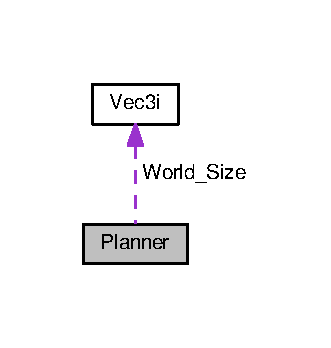
\includegraphics[width=159pt]{classPlanner__coll__graph}
\end{center}
\end{figure}
\subsection*{Public Member Functions}
\begin{DoxyCompactItemize}
\item 
\hyperlink{classPlanner_a828c56000cd1c514992c3f5a66c360eb}{Planner} (\hyperlink{structVec3i}{Vec3i})
\begin{DoxyCompactList}\small\item\em $<$ Public Access Specifier \end{DoxyCompactList}\item 
void \hyperlink{classPlanner_aba883f3b06c9ec1f50ff3715379b9315}{Set\+\_\+\+Heuristic} (std\+::function$<$ double(\hyperlink{structVec3i}{Vec3i}, \hyperlink{structVec3i}{Vec3i})$>$)
\begin{DoxyCompactList}\small\item\em Set\+\_\+\+Heuristic sets the Heuristic Behavior of neighbor Search. \end{DoxyCompactList}\item 
std\+::vector$<$ \hyperlink{structVec3i}{Vec3i} $>$ \hyperlink{classPlanner_a9d37842d3e18a53eadd201f8f9571a12}{find\+Path} (\hyperlink{structVec3i}{Vec3i}, \hyperlink{structVec3i}{Vec3i})
\begin{DoxyCompactList}\small\item\em find\+Path Finds the path from Start to Goal Point \end{DoxyCompactList}\item 
void \hyperlink{classPlanner_af25e70e04bccfebde65b2d5092e61633}{Add\+\_\+\+Collision} (\hyperlink{structVec3i}{Vec3i})
\begin{DoxyCompactList}\small\item\em Add\+\_\+\+Collision adds the Collision point to the walls list  of type \hyperlink{structVec3i}{Vec3i} contains the coordinates list of Obstacle. \end{DoxyCompactList}\item 
virtual \hyperlink{classPlanner_ac3db7cf113ad368fa6fce636b6e94abe}{$\sim$\+Planner} ()
\begin{DoxyCompactList}\small\item\em Destructor for \hyperlink{classPlanner}{Planner} Class. \end{DoxyCompactList}\end{DoxyCompactItemize}
\subsection*{Static Public Member Functions}
\begin{DoxyCompactItemize}
\item 
static double \hyperlink{classPlanner_a83d312b600eef6107513cbb39f083134}{Euclidean} (\hyperlink{structVec3i}{Vec3i}, \hyperlink{structVec3i}{Vec3i})
\begin{DoxyCompactList}\small\item\em Euclidean Distance Heuristic. \end{DoxyCompactList}\item 
static double \hyperlink{classPlanner_ad88eb501aedd40cdb3b60853ff7ad2b8}{Manhattan} (\hyperlink{structVec3i}{Vec3i}, \hyperlink{structVec3i}{Vec3i})
\begin{DoxyCompactList}\small\item\em Manhattan Distance Heuristic. \end{DoxyCompactList}\end{DoxyCompactItemize}
\subsection*{Public Attributes}
\begin{DoxyCompactItemize}
\item 
std\+::function$<$ double(\hyperlink{structVec3i}{Vec3i}, \hyperlink{structVec3i}{Vec3i})$>$ \hyperlink{classPlanner_a56d3e7453675b3f8be6e02e75ff2065e}{heuristic}
\item 
std\+::vector$<$ \hyperlink{structVec3i}{Vec3i} $>$ \hyperlink{classPlanner_a559fdca30a83a0da76d0538c8fe97379}{direction}
\item 
std\+::vector$<$ \hyperlink{structVec3i}{Vec3i} $>$ {\bfseries walls}\hypertarget{classPlanner_a44b47ff3ddda4a5d270000b69737970f}{}\label{classPlanner_a44b47ff3ddda4a5d270000b69737970f}

\item 
\hyperlink{structVec3i}{Vec3i} \hyperlink{classPlanner_a27c77443f0cf3e6b5197c0c3af56c3ca}{World\+\_\+\+Size}
\end{DoxyCompactItemize}


\subsection{Detailed Description}
Declaration of Class \hyperlink{classPlanner}{Planner}. 

\subsection{Constructor \& Destructor Documentation}
\index{Planner@{Planner}!Planner@{Planner}}
\index{Planner@{Planner}!Planner@{Planner}}
\subsubsection[{\texorpdfstring{Planner(\+Vec3i)}{Planner(Vec3i)}}]{\setlength{\rightskip}{0pt plus 5cm}Planner\+::\+Planner (
\begin{DoxyParamCaption}
\item[{{\bf Vec3i}}]{World\+\_\+\+Size\+\_\+}
\end{DoxyParamCaption}
)\hspace{0.3cm}{\ttfamily [explicit]}}\hypertarget{classPlanner_a828c56000cd1c514992c3f5a66c360eb}{}\label{classPlanner_a828c56000cd1c514992c3f5a66c360eb}


$<$ Public Access Specifier 

Constructor for class \hyperlink{classPlanner}{Planner} It initializes the \hyperlink{classPlanner}{Planner} with World Dimensions, Default Heuristic, Set of possible Directions.

Constructor for Class \hyperlink{classPlanner}{Planner}


\begin{DoxyParams}{Parameters}
{\em direction} & of type double initializes set of possible Directions \\
\hline
{\em World\+\_\+\+Size} & of size \hyperlink{structVec3i}{Vec3i} which stores the World Size \\
\hline
\end{DoxyParams}
$<$ Set default heuristic to Euclidean \index{Planner@{Planner}!````~Planner@{$\sim$\+Planner}}
\index{````~Planner@{$\sim$\+Planner}!Planner@{Planner}}
\subsubsection[{\texorpdfstring{$\sim$\+Planner()}{~Planner()}}]{\setlength{\rightskip}{0pt plus 5cm}Planner\+::$\sim$\+Planner (
\begin{DoxyParamCaption}
{}
\end{DoxyParamCaption}
)\hspace{0.3cm}{\ttfamily [virtual]}}\hypertarget{classPlanner_ac3db7cf113ad368fa6fce636b6e94abe}{}\label{classPlanner_ac3db7cf113ad368fa6fce636b6e94abe}


Destructor for \hyperlink{classPlanner}{Planner} Class. 

Destructor for \hyperlink{classPlanner}{Planner} Class 

\subsection{Member Function Documentation}
\index{Planner@{Planner}!Add\+\_\+\+Collision@{Add\+\_\+\+Collision}}
\index{Add\+\_\+\+Collision@{Add\+\_\+\+Collision}!Planner@{Planner}}
\subsubsection[{\texorpdfstring{Add\+\_\+\+Collision(\+Vec3i)}{Add_Collision(Vec3i)}}]{\setlength{\rightskip}{0pt plus 5cm}void Planner\+::\+Add\+\_\+\+Collision (
\begin{DoxyParamCaption}
\item[{{\bf Vec3i}}]{coordinates\+\_\+}
\end{DoxyParamCaption}
)}\hypertarget{classPlanner_af25e70e04bccfebde65b2d5092e61633}{}\label{classPlanner_af25e70e04bccfebde65b2d5092e61633}


Add\+\_\+\+Collision adds the Collision point to the walls list  of type \hyperlink{structVec3i}{Vec3i} contains the coordinates list of Obstacle. 

Add\+\_\+\+Collision adds the Nodes to Obstacle List

\begin{DoxyReturn}{Returns}
void 
\end{DoxyReturn}
\index{Planner@{Planner}!Euclidean@{Euclidean}}
\index{Euclidean@{Euclidean}!Planner@{Planner}}
\subsubsection[{\texorpdfstring{Euclidean(\+Vec3i, Vec3i)}{Euclidean(Vec3i, Vec3i)}}]{\setlength{\rightskip}{0pt plus 5cm}double Planner\+::\+Euclidean (
\begin{DoxyParamCaption}
\item[{{\bf Vec3i}}]{Now\+\_\+, }
\item[{{\bf Vec3i}}]{Neighbor\+\_\+}
\end{DoxyParamCaption}
)\hspace{0.3cm}{\ttfamily [static]}}\hypertarget{classPlanner_a83d312b600eef6107513cbb39f083134}{}\label{classPlanner_a83d312b600eef6107513cbb39f083134}


Euclidean Distance Heuristic. 

Euclidean is a Euclidean Distance Heuristic function.


\begin{DoxyParams}{Parameters}
{\em Now\+\_\+} & has type \hyperlink{structVec3i}{Vec3i} struct \\
\hline
{\em Neighbor\+\_\+} & has type \hyperlink{structVec3i}{Vec3i} struct \\
\hline
\end{DoxyParams}
\begin{DoxyReturn}{Returns}
double type Euclidean Distance between two points 
\end{DoxyReturn}
\index{Planner@{Planner}!find\+Path@{find\+Path}}
\index{find\+Path@{find\+Path}!Planner@{Planner}}
\subsubsection[{\texorpdfstring{find\+Path(\+Vec3i, Vec3i)}{findPath(Vec3i, Vec3i)}}]{\setlength{\rightskip}{0pt plus 5cm}std\+::vector$<$ {\bf Vec3i} $>$ Planner\+::find\+Path (
\begin{DoxyParamCaption}
\item[{{\bf Vec3i}}]{Start\+\_\+, }
\item[{{\bf Vec3i}}]{Goal\+\_\+}
\end{DoxyParamCaption}
)}\hypertarget{classPlanner_a9d37842d3e18a53eadd201f8f9571a12}{}\label{classPlanner_a9d37842d3e18a53eadd201f8f9571a12}


find\+Path Finds the path from Start to Goal Point 

find\+Path Plans the Path from Start to Goal Point


\begin{DoxyParams}{Parameters}
{\em Start\+\_\+} & of type \hyperlink{structVec3i}{Vec3i} struct which stores Start point coordinates \\
\hline
{\em Goal\+\_\+} & of type \hyperlink{structVec3i}{Vec3i} struct which store Goal point coordinates \\
\hline
\end{DoxyParams}
\begin{DoxyReturn}{Returns}
vector of \hyperlink{structVec3i}{Vec3i} type which contains Path from start to goal 
\end{DoxyReturn}
$<$ Set Current \hyperlink{structNode}{Node} pointer as Null pointer

$<$ Initialize the Open \& Closed Sets

$<$ Insert Start node to Open Set

Set current node pointer to First node of Open Set

Search for the node with least F value and set it as Current \hyperlink{structNode}{Node}

If Current \hyperlink{structNode}{Node} is Goal, Then Stop Searching

Insert Current \hyperlink{structNode}{Node} to the Closed Set

Remove Current \hyperlink{structNode}{Node} from Open Set

From all movable directions, check the neighbors

Check if Collision Happens

Find F value of Neighbor

Set Parent \hyperlink{structNode}{Node} to Successor \hyperlink{structNode}{Node}

Set G value of Successor

Print Path Not Found if Open List is Empty

Store Path from Start to Goal in path vector

$<$ Return Calculated path \index{Planner@{Planner}!Manhattan@{Manhattan}}
\index{Manhattan@{Manhattan}!Planner@{Planner}}
\subsubsection[{\texorpdfstring{Manhattan(\+Vec3i, Vec3i)}{Manhattan(Vec3i, Vec3i)}}]{\setlength{\rightskip}{0pt plus 5cm}double Planner\+::\+Manhattan (
\begin{DoxyParamCaption}
\item[{{\bf Vec3i}}]{Now\+\_\+, }
\item[{{\bf Vec3i}}]{Neighbor\+\_\+}
\end{DoxyParamCaption}
)\hspace{0.3cm}{\ttfamily [static]}}\hypertarget{classPlanner_ad88eb501aedd40cdb3b60853ff7ad2b8}{}\label{classPlanner_ad88eb501aedd40cdb3b60853ff7ad2b8}


Manhattan Distance Heuristic. 

Manhattan is a Manhattan Distance Heuristic function.


\begin{DoxyParams}{Parameters}
{\em Now\+\_\+} & has type \hyperlink{structVec3i}{Vec3i} struct \\
\hline
{\em Neighbor\+\_\+} & has type \hyperlink{structVec3i}{Vec3i} struct \\
\hline
\end{DoxyParams}
\begin{DoxyReturn}{Returns}
double type Manhattan Distance between two points 
\end{DoxyReturn}
\index{Planner@{Planner}!Set\+\_\+\+Heuristic@{Set\+\_\+\+Heuristic}}
\index{Set\+\_\+\+Heuristic@{Set\+\_\+\+Heuristic}!Planner@{Planner}}
\subsubsection[{\texorpdfstring{Set\+\_\+\+Heuristic(std\+::function$<$ double(\+Vec3i, Vec3i)$>$)}{Set_Heuristic(std::function< double(Vec3i, Vec3i)>)}}]{\setlength{\rightskip}{0pt plus 5cm}void Planner\+::\+Set\+\_\+\+Heuristic (
\begin{DoxyParamCaption}
\item[{std\+::function$<$ double({\bf Vec3i}, {\bf Vec3i})$>$}]{heuristic\+\_\+}
\end{DoxyParamCaption}
)}\hypertarget{classPlanner_aba883f3b06c9ec1f50ff3715379b9315}{}\label{classPlanner_aba883f3b06c9ec1f50ff3715379b9315}


Set\+\_\+\+Heuristic sets the Heuristic Behavior of neighbor Search. 

Set\+\_\+\+Heuristic sets the Heuristic Function


\begin{DoxyParams}{Parameters}
{\em heuristic} & builds heuristic given a heuristic function input \\
\hline
\end{DoxyParams}
\begin{DoxyReturn}{Returns}
void 
\end{DoxyReturn}


\subsection{Member Data Documentation}
\index{Planner@{Planner}!direction@{direction}}
\index{direction@{direction}!Planner@{Planner}}
\subsubsection[{\texorpdfstring{direction}{direction}}]{\setlength{\rightskip}{0pt plus 5cm}std\+::vector$<${\bf Vec3i}$>$ Planner\+::direction}\hypertarget{classPlanner_a559fdca30a83a0da76d0538c8fe97379}{}\label{classPlanner_a559fdca30a83a0da76d0538c8fe97379}
direction contains direction of movement from current to neighbor node. walls contains all Obstacle Nodes \index{Planner@{Planner}!heuristic@{heuristic}}
\index{heuristic@{heuristic}!Planner@{Planner}}
\subsubsection[{\texorpdfstring{heuristic}{heuristic}}]{\setlength{\rightskip}{0pt plus 5cm}std\+::function$<$double({\bf Vec3i}, {\bf Vec3i})$>$ Planner\+::heuristic}\hypertarget{classPlanner_a56d3e7453675b3f8be6e02e75ff2065e}{}\label{classPlanner_a56d3e7453675b3f8be6e02e75ff2065e}
Heuristic Function \index{Planner@{Planner}!World\+\_\+\+Size@{World\+\_\+\+Size}}
\index{World\+\_\+\+Size@{World\+\_\+\+Size}!Planner@{Planner}}
\subsubsection[{\texorpdfstring{World\+\_\+\+Size}{World_Size}}]{\setlength{\rightskip}{0pt plus 5cm}{\bf Vec3i} Planner\+::\+World\+\_\+\+Size}\hypertarget{classPlanner_a27c77443f0cf3e6b5197c0c3af56c3ca}{}\label{classPlanner_a27c77443f0cf3e6b5197c0c3af56c3ca}
World\+\_\+\+Size of return type \hyperlink{structVec3i}{Vec3i} struct contains world dimensions 

The documentation for this class was generated from the following files\+:\begin{DoxyCompactItemize}
\item 
include/\hyperlink{Planner_8h}{Planner.\+h}\item 
app/\hyperlink{Planner_8cpp}{Planner.\+cpp}\end{DoxyCompactItemize}

\hypertarget{structVec3i}{}\section{Vec3i Struct Reference}
\label{structVec3i}\index{Vec3i@{Vec3i}}


\hyperlink{structVec3i}{Vec3i} of type Struct which Builds points with x,y,z values.  




{\ttfamily \#include $<$Planner.\+h$>$}

\subsection*{Public Member Functions}
\begin{DoxyCompactItemize}
\item 
bool \hyperlink{structVec3i_abc87945692cbc7cd92b855a5d3fcd668}{operator==} (const \hyperlink{structVec3i}{Vec3i} \&coordinates\+\_\+)
\begin{DoxyCompactList}\small\item\em operator of return type boolean from \hyperlink{structVec3i}{Vec3i} struct It compares the X,Y,Z, values of given coordinate with reference \end{DoxyCompactList}\end{DoxyCompactItemize}
\subsection*{Public Attributes}
\begin{DoxyCompactItemize}
\item 
int \hyperlink{structVec3i_a00db3692921caac03a0e0fd3d8f619c9}{x}
\item 
int {\bfseries y}\hypertarget{structVec3i_a2d63847534d5ae0829f5e0e69d93d02c}{}\label{structVec3i_a2d63847534d5ae0829f5e0e69d93d02c}

\item 
int {\bfseries z}\hypertarget{structVec3i_a5b773400513d24edae3f7e806651a21c}{}\label{structVec3i_a5b773400513d24edae3f7e806651a21c}

\end{DoxyCompactItemize}


\subsection{Detailed Description}
\hyperlink{structVec3i}{Vec3i} of type Struct which Builds points with x,y,z values. 

\subsection{Member Function Documentation}
\index{Vec3i@{Vec3i}!operator==@{operator==}}
\index{operator==@{operator==}!Vec3i@{Vec3i}}
\subsubsection[{\texorpdfstring{operator==(const Vec3i \&coordinates\+\_\+)}{operator==(const Vec3i &coordinates_)}}]{\setlength{\rightskip}{0pt plus 5cm}bool Vec3i\+::operator== (
\begin{DoxyParamCaption}
\item[{const {\bf Vec3i} \&}]{coordinates\+\_\+}
\end{DoxyParamCaption}
)}\hypertarget{structVec3i_abc87945692cbc7cd92b855a5d3fcd668}{}\label{structVec3i_abc87945692cbc7cd92b855a5d3fcd668}


operator of return type boolean from \hyperlink{structVec3i}{Vec3i} struct It compares the X,Y,Z, values of given coordinate with reference 

operator of type boolean

\begin{DoxyReturn}{Returns}
boolean true if coordinate matches the reference else return false 
\end{DoxyReturn}


\subsection{Member Data Documentation}
\index{Vec3i@{Vec3i}!x@{x}}
\index{x@{x}!Vec3i@{Vec3i}}
\subsubsection[{\texorpdfstring{x}{x}}]{\setlength{\rightskip}{0pt plus 5cm}int Vec3i\+::x}\hypertarget{structVec3i_a00db3692921caac03a0e0fd3d8f619c9}{}\label{structVec3i_a00db3692921caac03a0e0fd3d8f619c9}
x,y,z of type integer 

The documentation for this struct was generated from the following files\+:\begin{DoxyCompactItemize}
\item 
include/\hyperlink{Planner_8h}{Planner.\+h}\item 
app/\hyperlink{Planner_8cpp}{Planner.\+cpp}\end{DoxyCompactItemize}

\chapter{File Documentation}
\hypertarget{Build__Map_8cpp}{}\section{app/\+Build\+\_\+\+Map.cpp File Reference}
\label{Build__Map_8cpp}\index{app/\+Build\+\_\+\+Map.\+cpp@{app/\+Build\+\_\+\+Map.\+cpp}}


This File contains the code for \hyperlink{classBuild__Map}{Build\+\_\+\+Map} class which Discretizes the World using resolution values and marks obstacle positions in the workspace. Converts points from World to Discretized Workspace and vice versa.  


{\ttfamily \#include $<$iostream$>$}\\*
{\ttfamily \#include $<$cmath$>$}\\*
{\ttfamily \#include $<$vector$>$}\\*
{\ttfamily \#include \char`\"{}../include/\+Build\+\_\+\+Map.\+h\char`\"{}}\\*
Include dependency graph for Build\+\_\+\+Map.\+cpp\+:\nopagebreak
\begin{figure}[H]
\begin{center}
\leavevmode
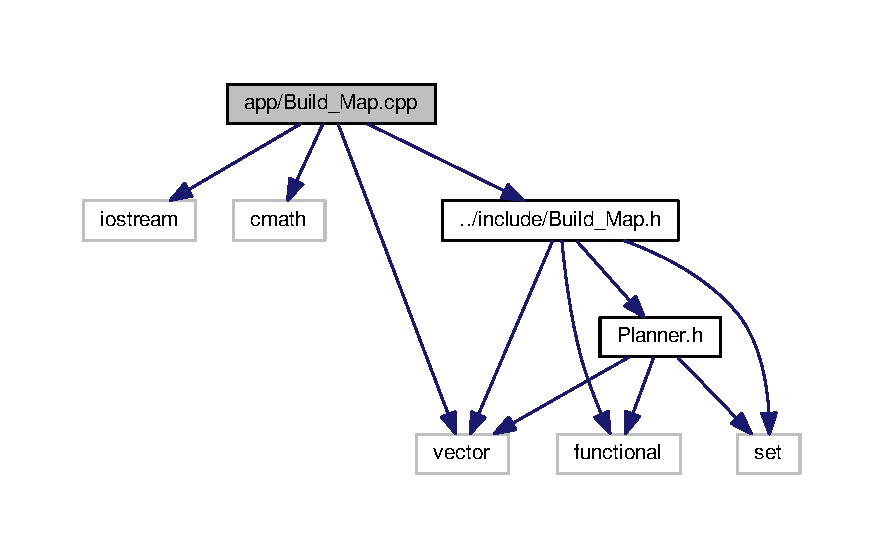
\includegraphics[width=350pt]{Build__Map_8cpp__incl}
\end{center}
\end{figure}


\subsection{Detailed Description}
This File contains the code for \hyperlink{classBuild__Map}{Build\+\_\+\+Map} class which Discretizes the World using resolution values and marks obstacle positions in the workspace. Converts points from World to Discretized Workspace and vice versa. 

\begin{DoxyAuthor}{Author}
Vaibhav Bhilare 
\end{DoxyAuthor}
\begin{DoxyCopyright}{Copyright}
2017, Vaibhav Bhilare
\end{DoxyCopyright}
M\+IT License Copyright (c) 2017 Vaibhav Bhilare

Permission is hereby granted, free of charge, to any person obtaining a copy of this software and associated documentation files (the \char`\"{}\+Software\char`\"{}), to deal in the Software without restriction, including without limitation the rights to use, copy, modify, merge, publish, distribute, sublicense, and/or sell copies of the Software, and to permit persons to whom the Software is furnished to do so, subject to the following conditions\+:

The above copyright notice and this permission notice shall be included in all copies or substantial portions of the Software.

T\+HE S\+O\+F\+T\+W\+A\+RE IS P\+R\+O\+V\+I\+D\+ED \char`\"{}\+A\+S I\+S\char`\"{}, W\+I\+T\+H\+O\+UT W\+A\+R\+R\+A\+N\+TY OF A\+NY K\+I\+ND, E\+X\+P\+R\+E\+SS OR I\+M\+P\+L\+I\+ED, I\+N\+C\+L\+U\+D\+I\+NG B\+UT N\+OT L\+I\+M\+I\+T\+ED TO T\+HE W\+A\+R\+R\+A\+N\+T\+I\+ES OF M\+E\+R\+C\+H\+A\+N\+T\+A\+B\+I\+L\+I\+TY, F\+I\+T\+N\+E\+SS F\+OR A P\+A\+R\+T\+I\+C\+U\+L\+AR P\+U\+R\+P\+O\+SE A\+ND N\+O\+N\+I\+N\+F\+R\+I\+N\+G\+E\+M\+E\+NT. IN NO E\+V\+E\+NT S\+H\+A\+LL T\+HE A\+U\+T\+H\+O\+RS OR C\+O\+P\+Y\+R\+I\+G\+HT H\+O\+L\+D\+E\+RS BE L\+I\+A\+B\+LE F\+OR A\+NY C\+L\+A\+IM, D\+A\+M\+A\+G\+ES OR O\+T\+H\+ER L\+I\+A\+B\+I\+L\+I\+TY, W\+H\+E\+T\+H\+ER IN AN A\+C\+T\+I\+ON OF C\+O\+N\+T\+R\+A\+CT, T\+O\+RT OR O\+T\+H\+E\+R\+W\+I\+SE, A\+R\+I\+S\+I\+NG F\+R\+OM, O\+UT OF OR IN C\+O\+N\+N\+E\+C\+T\+I\+ON W\+I\+TH T\+HE S\+O\+F\+T\+W\+A\+RE OR T\+HE U\+SE OR O\+T\+H\+ER D\+E\+A\+L\+I\+N\+GS IN T\+HE S\+O\+F\+T\+W\+A\+RE. 
\hypertarget{main_8cpp}{}\section{app/main.cpp File Reference}
\label{main_8cpp}\index{app/main.\+cpp@{app/main.\+cpp}}


This project builds a discrete 3-\/D map from environment information and Implements the A$\ast$ algorithm to plan the path from Start to Goal Point.  


{\ttfamily \#include $<$iostream$>$}\\*
{\ttfamily \#include $<$vector$>$}\\*
{\ttfamily \#include $<$cmath$>$}\\*
{\ttfamily \#include \char`\"{}../include/\+Planner.\+h\char`\"{}}\\*
{\ttfamily \#include \char`\"{}../include/\+Build\+\_\+\+Map.\+h\char`\"{}}\\*
Include dependency graph for main.\+cpp\+:\nopagebreak
\begin{figure}[H]
\begin{center}
\leavevmode
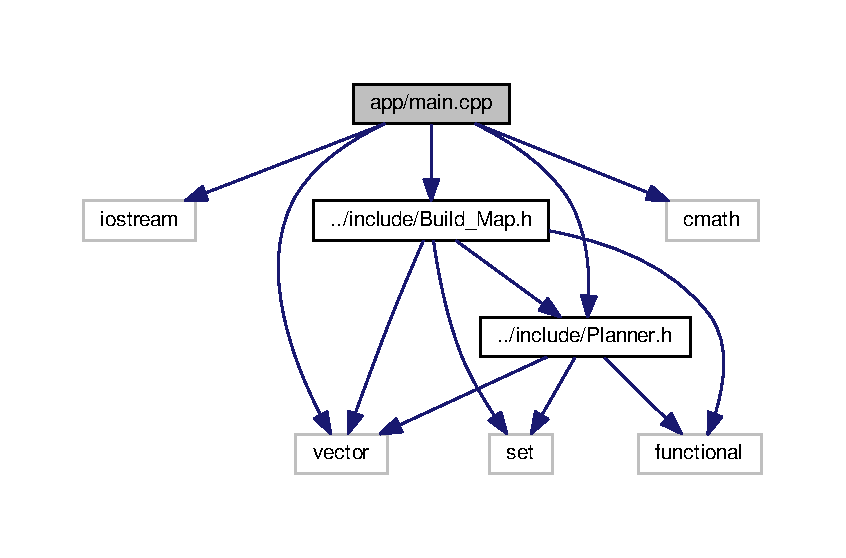
\includegraphics[width=350pt]{main_8cpp__incl}
\end{center}
\end{figure}
\subsection*{Functions}
\begin{DoxyCompactItemize}
\item 
int \hyperlink{main_8cpp_ae66f6b31b5ad750f1fe042a706a4e3d4}{main} ()
\begin{DoxyCompactList}\small\item\em main method \end{DoxyCompactList}\end{DoxyCompactItemize}


\subsection{Detailed Description}
This project builds a discrete 3-\/D map from environment information and Implements the A$\ast$ algorithm to plan the path from Start to Goal Point. 

\begin{DoxyAuthor}{Author}
Vaibhav Bhilare 
\end{DoxyAuthor}
\begin{DoxyCopyright}{Copyright}
2017, Vaibhav Bhilare
\end{DoxyCopyright}
M\+IT License Copyright (c) 2017 Vaibhav Bhilare

Permission is hereby granted, free of charge, to any person obtaining a copy of this software and associated documentation files (the \char`\"{}\+Software\char`\"{}), to deal in the Software without restriction, including without limitation the rights to use, copy, modify, merge, publish, distribute, sublicense, and/or sell copies of the Software, and to permit persons to whom the Software is furnished to do so, subject to the following conditions\+:

The above copyright notice and this permission notice shall be included in all copies or substantial portions of the Software.

T\+HE S\+O\+F\+T\+W\+A\+RE IS P\+R\+O\+V\+I\+D\+ED \char`\"{}\+A\+S I\+S\char`\"{}, W\+I\+T\+H\+O\+UT W\+A\+R\+R\+A\+N\+TY OF A\+NY K\+I\+ND, E\+X\+P\+R\+E\+SS OR I\+M\+P\+L\+I\+ED, I\+N\+C\+L\+U\+D\+I\+NG B\+UT N\+OT L\+I\+M\+I\+T\+ED TO T\+HE W\+A\+R\+R\+A\+N\+T\+I\+ES OF M\+E\+R\+C\+H\+A\+N\+T\+A\+B\+I\+L\+I\+TY, F\+I\+T\+N\+E\+SS F\+OR A P\+A\+R\+T\+I\+C\+U\+L\+AR P\+U\+R\+P\+O\+SE A\+ND N\+O\+N\+I\+N\+F\+R\+I\+N\+G\+E\+M\+E\+NT. IN NO E\+V\+E\+NT S\+H\+A\+LL T\+HE A\+U\+T\+H\+O\+RS OR C\+O\+P\+Y\+R\+I\+G\+HT H\+O\+L\+D\+E\+RS BE L\+I\+A\+B\+LE F\+OR A\+NY C\+L\+A\+IM, D\+A\+M\+A\+G\+ES OR O\+T\+H\+ER L\+I\+A\+B\+I\+L\+I\+TY, W\+H\+E\+T\+H\+ER IN AN A\+C\+T\+I\+ON OF C\+O\+N\+T\+R\+A\+CT, T\+O\+RT OR O\+T\+H\+E\+R\+W\+I\+SE, A\+R\+I\+S\+I\+NG F\+R\+OM, O\+UT OF OR IN C\+O\+N\+N\+E\+C\+T\+I\+ON W\+I\+TH T\+HE S\+O\+F\+T\+W\+A\+RE OR T\+HE U\+SE OR O\+T\+H\+ER D\+E\+A\+L\+I\+N\+GS IN T\+HE S\+O\+F\+T\+W\+A\+RE. 

\subsection{Function Documentation}
\index{main.\+cpp@{main.\+cpp}!main@{main}}
\index{main@{main}!main.\+cpp@{main.\+cpp}}
\subsubsection[{\texorpdfstring{main()}{main()}}]{\setlength{\rightskip}{0pt plus 5cm}int main (
\begin{DoxyParamCaption}
{}
\end{DoxyParamCaption}
)}\hypertarget{main_8cpp_ae66f6b31b5ad750f1fe042a706a4e3d4}{}\label{main_8cpp_ae66f6b31b5ad750f1fe042a706a4e3d4}


main method 

--Includes-- Takes the World Boundary and Obstacle Data. Sends them to Build a Discrete 3-\/D Map. This map is sent to the planner which then plans the path from Start to Goal point using A$\ast$ \hyperlink{classPlanner}{Planner}.

\begin{DoxyReturn}{Returns}
0 
\end{DoxyReturn}
Initialize the x,y,z resolution values. Initialize the Margin Value for Robot Dimensions. Initialize the World Boundary and Obstacles.

$<$ Initialize the x,y resolution.

$<$ Initialize the z resolution.

$<$ Initialize the margin value for robot dimensions.

Initialize the World Boundary in \{xmin,ymin,zmin,xmax,ymax,zmax\} format.

Initialize the Obstacles in \{xmin,ymin,zmin,xmax,ymax,zmax\} format.

Create an Instance of the \hyperlink{classBuild__Map}{Build\+\_\+\+Map} Class named Map.

Store the Discretized World Dimensions in World.

Create an Instance of the \hyperlink{classPlanner}{Planner} Class named Plan.

Add the nodes inside Obstacles to Collision List.

Set Heuristic Function to Euclidean or Manhattan (Default Euclidean).

$<$ Initialize Start Point.

$<$ Initialize Goal Point.

Check whether the Start or Goal points lie outside the World.

If Start and Goal Points are inside the world, find their positions in the discretized world.

Plan the Path from Start to Goal using find\+Path. Get the value in path.

Print the Path

$<$ Return 0. 
\hypertarget{Planner_8cpp}{}\section{app/\+Planner.cpp File Reference}
\label{Planner_8cpp}\index{app/\+Planner.\+cpp@{app/\+Planner.\+cpp}}


This file contains the code for \hyperlink{classPlanner}{Planner} Class which takes the Environment data built by the \hyperlink{classBuild__Map}{Build\+\_\+\+Map} Class and Uses A$\ast$ to plan the Shortest Path while avoiding all Obstacles.  


{\ttfamily \#include $<$iostream$>$}\\*
{\ttfamily \#include $<$algorithm$>$}\\*
{\ttfamily \#include $<$cmath$>$}\\*
{\ttfamily \#include $<$utility$>$}\\*
{\ttfamily \#include $<$vector$>$}\\*
{\ttfamily \#include $<$set$>$}\\*
{\ttfamily \#include \char`\"{}../include/\+Planner.\+h\char`\"{}}\\*
Include dependency graph for Planner.\+cpp\+:\nopagebreak
\begin{figure}[H]
\begin{center}
\leavevmode
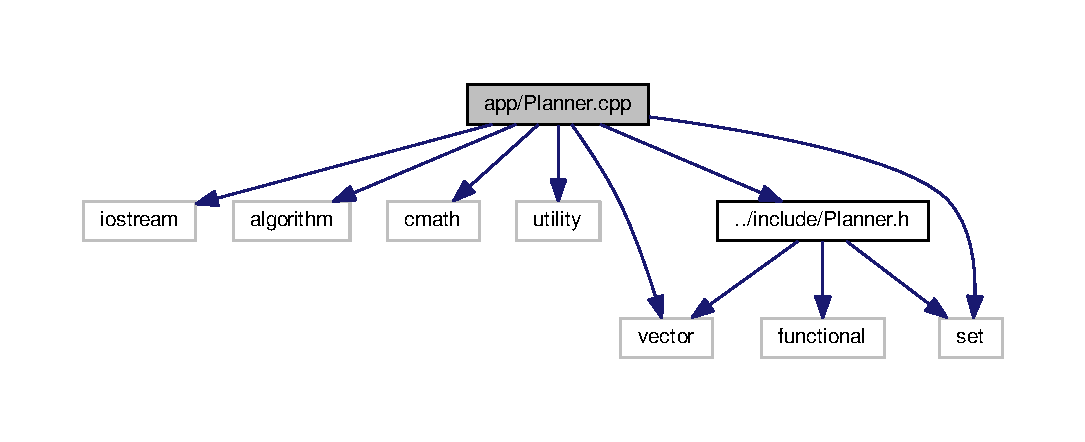
\includegraphics[width=350pt]{Planner_8cpp__incl}
\end{center}
\end{figure}
\subsection*{Functions}
\begin{DoxyCompactItemize}
\item 
\hyperlink{structVec3i}{Vec3i} \hyperlink{Planner_8cpp_a80ad1b1e6b2cd53eaf29cc875d3d4470}{operator+} (const \hyperlink{structVec3i}{Vec3i} \&left\+\_\+, const \hyperlink{structVec3i}{Vec3i} \&right\+\_\+)
\begin{DoxyCompactList}\small\item\em Addition Operator of return type \hyperlink{structVec3i}{Vec3i} struct It adds corresonding X,Y,Z values of two \hyperlink{structVec3i}{Vec3i} structs and returns a new \hyperlink{structVec3i}{Vec3i} Struct. \end{DoxyCompactList}\end{DoxyCompactItemize}


\subsection{Detailed Description}
This file contains the code for \hyperlink{classPlanner}{Planner} Class which takes the Environment data built by the \hyperlink{classBuild__Map}{Build\+\_\+\+Map} Class and Uses A$\ast$ to plan the Shortest Path while avoiding all Obstacles. 

\begin{DoxyAuthor}{Author}
Vaibhav Bhilare 
\end{DoxyAuthor}
\begin{DoxyCopyright}{Copyright}
2017, Vaibhav Bhilare
\end{DoxyCopyright}
M\+IT License Copyright (c) 2017 Vaibhav Bhilare

Permission is hereby granted, free of charge, to any person obtaining a copy of this software and associated documentation files (the \char`\"{}\+Software\char`\"{}), to deal in the Software without restriction, including without limitation the rights to use, copy, modify, merge, publish, distribute, sublicense, and/or sell copies of the Software, and to permit persons to whom the Software is furnished to do so, subject to the following conditions\+:

The above copyright notice and this permission notice shall be included in all copies or substantial portions of the Software.

T\+HE S\+O\+F\+T\+W\+A\+RE IS P\+R\+O\+V\+I\+D\+ED \char`\"{}\+A\+S I\+S\char`\"{}, W\+I\+T\+H\+O\+UT W\+A\+R\+R\+A\+N\+TY OF A\+NY K\+I\+ND, E\+X\+P\+R\+E\+SS OR I\+M\+P\+L\+I\+ED, I\+N\+C\+L\+U\+D\+I\+NG B\+UT N\+OT L\+I\+M\+I\+T\+ED TO T\+HE W\+A\+R\+R\+A\+N\+T\+I\+ES OF M\+E\+R\+C\+H\+A\+N\+T\+A\+B\+I\+L\+I\+TY, F\+I\+T\+N\+E\+SS F\+OR A P\+A\+R\+T\+I\+C\+U\+L\+AR P\+U\+R\+P\+O\+SE A\+ND N\+O\+N\+I\+N\+F\+R\+I\+N\+G\+E\+M\+E\+NT. IN NO E\+V\+E\+NT S\+H\+A\+LL T\+HE A\+U\+T\+H\+O\+RS OR C\+O\+P\+Y\+R\+I\+G\+HT H\+O\+L\+D\+E\+RS BE L\+I\+A\+B\+LE F\+OR A\+NY C\+L\+A\+IM, D\+A\+M\+A\+G\+ES OR O\+T\+H\+ER L\+I\+A\+B\+I\+L\+I\+TY, W\+H\+E\+T\+H\+ER IN AN A\+C\+T\+I\+ON OF C\+O\+N\+T\+R\+A\+CT, T\+O\+RT OR O\+T\+H\+E\+R\+W\+I\+SE, A\+R\+I\+S\+I\+NG F\+R\+OM, O\+UT OF OR IN C\+O\+N\+N\+E\+C\+T\+I\+ON W\+I\+TH T\+HE S\+O\+F\+T\+W\+A\+RE OR T\+HE U\+SE OR O\+T\+H\+ER D\+E\+A\+L\+I\+N\+GS IN T\+HE S\+O\+F\+T\+W\+A\+RE. 

\subsection{Function Documentation}
\index{Planner.\+cpp@{Planner.\+cpp}!operator+@{operator+}}
\index{operator+@{operator+}!Planner.\+cpp@{Planner.\+cpp}}
\subsubsection[{\texorpdfstring{operator+(const Vec3i \&left\+\_\+, const Vec3i \&right\+\_\+)}{operator+(const Vec3i &left_, const Vec3i &right_)}}]{\setlength{\rightskip}{0pt plus 5cm}{\bf Vec3i} operator+ (
\begin{DoxyParamCaption}
\item[{const {\bf Vec3i} \&}]{left\+\_\+, }
\item[{const {\bf Vec3i} \&}]{right\+\_\+}
\end{DoxyParamCaption}
)}\hypertarget{Planner_8cpp_a80ad1b1e6b2cd53eaf29cc875d3d4470}{}\label{Planner_8cpp_a80ad1b1e6b2cd53eaf29cc875d3d4470}


Addition Operator of return type \hyperlink{structVec3i}{Vec3i} struct It adds corresonding X,Y,Z values of two \hyperlink{structVec3i}{Vec3i} structs and returns a new \hyperlink{structVec3i}{Vec3i} Struct. 

\begin{DoxyReturn}{Returns}
\hyperlink{structVec3i}{Vec3i} type Struct 
\end{DoxyReturn}

\hypertarget{Build__Map_8h}{}\section{include/\+Build\+\_\+\+Map.h File Reference}
\label{Build__Map_8h}\index{include/\+Build\+\_\+\+Map.\+h@{include/\+Build\+\_\+\+Map.\+h}}


This File contains the declarations of variables and methods for \hyperlink{classBuild__Map}{Build\+\_\+\+Map} class which Discretizes the World using resolution values and marks obstacle positions in the workspace. Converts points from World to Discretized Workspace and vice versa.  


{\ttfamily \#include $<$vector$>$}\\*
{\ttfamily \#include $<$functional$>$}\\*
{\ttfamily \#include $<$set$>$}\\*
{\ttfamily \#include \char`\"{}Planner.\+h\char`\"{}}\\*
Include dependency graph for Build\+\_\+\+Map.\+h\+:\nopagebreak
\begin{figure}[H]
\begin{center}
\leavevmode
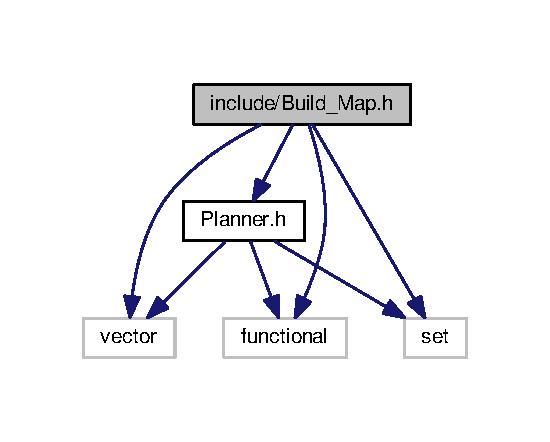
\includegraphics[width=264pt]{Build__Map_8h__incl}
\end{center}
\end{figure}
This graph shows which files directly or indirectly include this file\+:\nopagebreak
\begin{figure}[H]
\begin{center}
\leavevmode
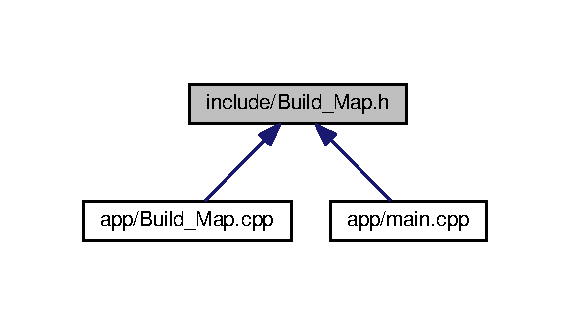
\includegraphics[width=274pt]{Build__Map_8h__dep__incl}
\end{center}
\end{figure}
\subsection*{Classes}
\begin{DoxyCompactItemize}
\item 
class \hyperlink{classBuild__Map}{Build\+\_\+\+Map}
\begin{DoxyCompactList}\small\item\em \hyperlink{classBuild__Map}{Build\+\_\+\+Map} class declaration. \end{DoxyCompactList}\end{DoxyCompactItemize}


\subsection{Detailed Description}
This File contains the declarations of variables and methods for \hyperlink{classBuild__Map}{Build\+\_\+\+Map} class which Discretizes the World using resolution values and marks obstacle positions in the workspace. Converts points from World to Discretized Workspace and vice versa. 

\begin{DoxyAuthor}{Author}
Vaibhav Bhilare 
\end{DoxyAuthor}
\begin{DoxyCopyright}{Copyright}
2017, Vaibhav Bhilare
\end{DoxyCopyright}
M\+IT License Copyright (c) 2017 Vaibhav Bhilare

Permission is hereby granted, free of charge, to any person obtaining a copy of this software and associated documentation files (the \char`\"{}\+Software\char`\"{}), to deal in the Software without restriction, including without limitation the rights to use, copy, modify, merge, publish, distribute, sublicense, and/or sell copies of the Software, and to permit persons to whom the Software is furnished to do so, subject to the following conditions\+:

The above copyright notice and this permission notice shall be included in all copies or substantial portions of the Software.

T\+HE S\+O\+F\+T\+W\+A\+RE IS P\+R\+O\+V\+I\+D\+ED \char`\"{}\+A\+S I\+S\char`\"{}, W\+I\+T\+H\+O\+UT W\+A\+R\+R\+A\+N\+TY OF A\+NY K\+I\+ND, E\+X\+P\+R\+E\+SS OR I\+M\+P\+L\+I\+ED, I\+N\+C\+L\+U\+D\+I\+NG B\+UT N\+OT L\+I\+M\+I\+T\+ED TO T\+HE W\+A\+R\+R\+A\+N\+T\+I\+ES OF M\+E\+R\+C\+H\+A\+N\+T\+A\+B\+I\+L\+I\+TY, F\+I\+T\+N\+E\+SS F\+OR A P\+A\+R\+T\+I\+C\+U\+L\+AR P\+U\+R\+P\+O\+SE A\+ND N\+O\+N\+I\+N\+F\+R\+I\+N\+G\+E\+M\+E\+NT. IN NO E\+V\+E\+NT S\+H\+A\+LL T\+HE A\+U\+T\+H\+O\+RS OR C\+O\+P\+Y\+R\+I\+G\+HT H\+O\+L\+D\+E\+RS BE L\+I\+A\+B\+LE F\+OR A\+NY C\+L\+A\+IM, D\+A\+M\+A\+G\+ES OR O\+T\+H\+ER L\+I\+A\+B\+I\+L\+I\+TY, W\+H\+E\+T\+H\+ER IN AN A\+C\+T\+I\+ON OF C\+O\+N\+T\+R\+A\+CT, T\+O\+RT OR O\+T\+H\+E\+R\+W\+I\+SE, A\+R\+I\+S\+I\+NG F\+R\+OM, O\+UT OF OR IN C\+O\+N\+N\+E\+C\+T\+I\+ON W\+I\+TH T\+HE S\+O\+F\+T\+W\+A\+RE OR T\+HE U\+SE OR O\+T\+H\+ER D\+E\+A\+L\+I\+N\+GS IN T\+HE S\+O\+F\+T\+W\+A\+RE. 
\hypertarget{Planner_8h}{}\section{include/\+Planner.h File Reference}
\label{Planner_8h}\index{include/\+Planner.\+h@{include/\+Planner.\+h}}


This file contains the variables and function declarations for \hyperlink{classPlanner}{Planner} Class which takes the Environment data built by the \hyperlink{classBuild__Map}{Build\+\_\+\+Map} Class and Uses A$\ast$ to plan the Shortest Path while avoiding all Obstacles.  


{\ttfamily \#include $<$vector$>$}\\*
{\ttfamily \#include $<$functional$>$}\\*
{\ttfamily \#include $<$set$>$}\\*
Include dependency graph for Planner.\+h\+:\nopagebreak
\begin{figure}[H]
\begin{center}
\leavevmode
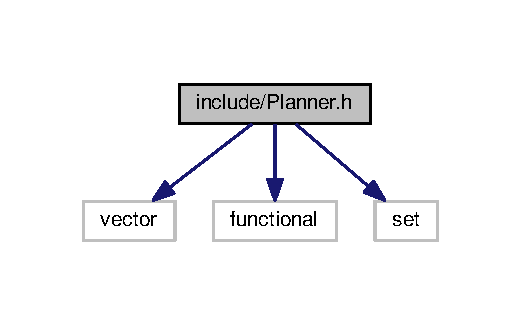
\includegraphics[width=250pt]{Planner_8h__incl}
\end{center}
\end{figure}
This graph shows which files directly or indirectly include this file\+:\nopagebreak
\begin{figure}[H]
\begin{center}
\leavevmode
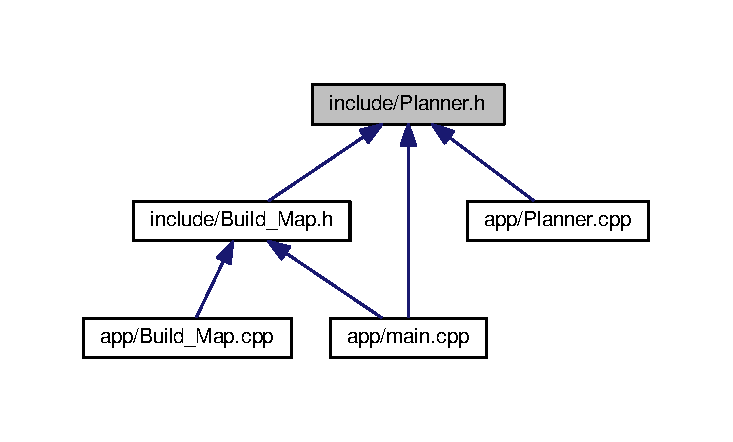
\includegraphics[width=350pt]{Planner_8h__dep__incl}
\end{center}
\end{figure}
\subsection*{Classes}
\begin{DoxyCompactItemize}
\item 
struct \hyperlink{structVec3i}{Vec3i}
\begin{DoxyCompactList}\small\item\em \hyperlink{structVec3i}{Vec3i} of type Struct which Builds points with x,y,z values. \end{DoxyCompactList}\item 
struct \hyperlink{structNode}{Node}
\begin{DoxyCompactList}\small\item\em \hyperlink{structNode}{Node} of type Struct which Stores Various Property values of the Nodes. \end{DoxyCompactList}\item 
class \hyperlink{classPlanner}{Planner}
\begin{DoxyCompactList}\small\item\em Declaration of Class \hyperlink{classPlanner}{Planner}. \end{DoxyCompactList}\end{DoxyCompactItemize}


\subsection{Detailed Description}
This file contains the variables and function declarations for \hyperlink{classPlanner}{Planner} Class which takes the Environment data built by the \hyperlink{classBuild__Map}{Build\+\_\+\+Map} Class and Uses A$\ast$ to plan the Shortest Path while avoiding all Obstacles. 

\begin{DoxyAuthor}{Author}
Vaibhav Bhilare 
\end{DoxyAuthor}
\begin{DoxyCopyright}{Copyright}
2017, Vaibhav Bhilare
\end{DoxyCopyright}
M\+IT License Copyright (c) 2017 Vaibhav Bhilare

Permission is hereby granted, free of charge, to any person obtaining a copy of this software and associated documentation files (the \char`\"{}\+Software\char`\"{}), to deal in the Software without restriction, including without limitation the rights to use, copy, modify, merge, publish, distribute, sublicense, and/or sell copies of the Software, and to permit persons to whom the Software is furnished to do so, subject to the following conditions\+:

The above copyright notice and this permission notice shall be included in all copies or substantial portions of the Software.

T\+HE S\+O\+F\+T\+W\+A\+RE IS P\+R\+O\+V\+I\+D\+ED \char`\"{}\+A\+S I\+S\char`\"{}, W\+I\+T\+H\+O\+UT W\+A\+R\+R\+A\+N\+TY OF A\+NY K\+I\+ND, E\+X\+P\+R\+E\+SS OR I\+M\+P\+L\+I\+ED, I\+N\+C\+L\+U\+D\+I\+NG B\+UT N\+OT L\+I\+M\+I\+T\+ED TO T\+HE W\+A\+R\+R\+A\+N\+T\+I\+ES OF M\+E\+R\+C\+H\+A\+N\+T\+A\+B\+I\+L\+I\+TY, F\+I\+T\+N\+E\+SS F\+OR A P\+A\+R\+T\+I\+C\+U\+L\+AR P\+U\+R\+P\+O\+SE A\+ND N\+O\+N\+I\+N\+F\+R\+I\+N\+G\+E\+M\+E\+NT. IN NO E\+V\+E\+NT S\+H\+A\+LL T\+HE A\+U\+T\+H\+O\+RS OR C\+O\+P\+Y\+R\+I\+G\+HT H\+O\+L\+D\+E\+RS BE L\+I\+A\+B\+LE F\+OR A\+NY C\+L\+A\+IM, D\+A\+M\+A\+G\+ES OR O\+T\+H\+ER L\+I\+A\+B\+I\+L\+I\+TY, W\+H\+E\+T\+H\+ER IN AN A\+C\+T\+I\+ON OF C\+O\+N\+T\+R\+A\+CT, T\+O\+RT OR O\+T\+H\+E\+R\+W\+I\+SE, A\+R\+I\+S\+I\+NG F\+R\+OM, O\+UT OF OR IN C\+O\+N\+N\+E\+C\+T\+I\+ON W\+I\+TH T\+HE S\+O\+F\+T\+W\+A\+RE OR T\+HE U\+SE OR O\+T\+H\+ER D\+E\+A\+L\+I\+N\+GS IN T\+HE S\+O\+F\+T\+W\+A\+RE. 
%--- End generated contents ---

% Index
\backmatter
\newpage
\phantomsection
\clearemptydoublepage
\addcontentsline{toc}{chapter}{Index}
\printindex

\end{document}
